\documentclass[parskip=full]{scrartcl}

\usepackage[T1]{fontenc}
\usepackage[ngerman]{babel}	
\usepackage[utf8]{inputenc}	

\usepackage{graphicx}
\usepackage{pdfpages}
\usepackage{float}
\usepackage[nooneline]{caption}
\usepackage{wrapfig}
\usepackage{pdfpages}
\usepackage{hyperref}	% Als letztes laden.
\hypersetup{
pdftitle={
	PSE: Entwurfsdokument},
bookmarks=true
}

\makeatletter
\renewcommand\paragraph{\@startsection{paragraph}{4}{\z@}%
	{-2.5ex\@plus -1ex \@minus -.25ex}%
	{1.25ex \@plus .25ex}%
	{\normalfont\normalsize\bfseries}}
\makeatother
\setcounter{secnumdepth}{5} % how many sectioning levels to assign numbers to
\setcounter{tocdepth}{5} 

\makeindex

\begin{document}
\title{Android-Go-App Entwurfsdokument}
\author{\\Dennis Bäuml,\\ Matthias Dressel,\\ Theresa Heine,\\ Victoria Karl, \\ Tarek Wilkening\\
	\\ \textbf{Betreuer:} \\Erik Burger, \\Axel Busch, \\Heiko Klare \\}
	
\date{\today}
\maketitle
\newpage
\tableofcontents
\newpage

\section{Grobentwurf}
\begin{figure}[h!]
     \centering
     \hspace*{-0.5cm}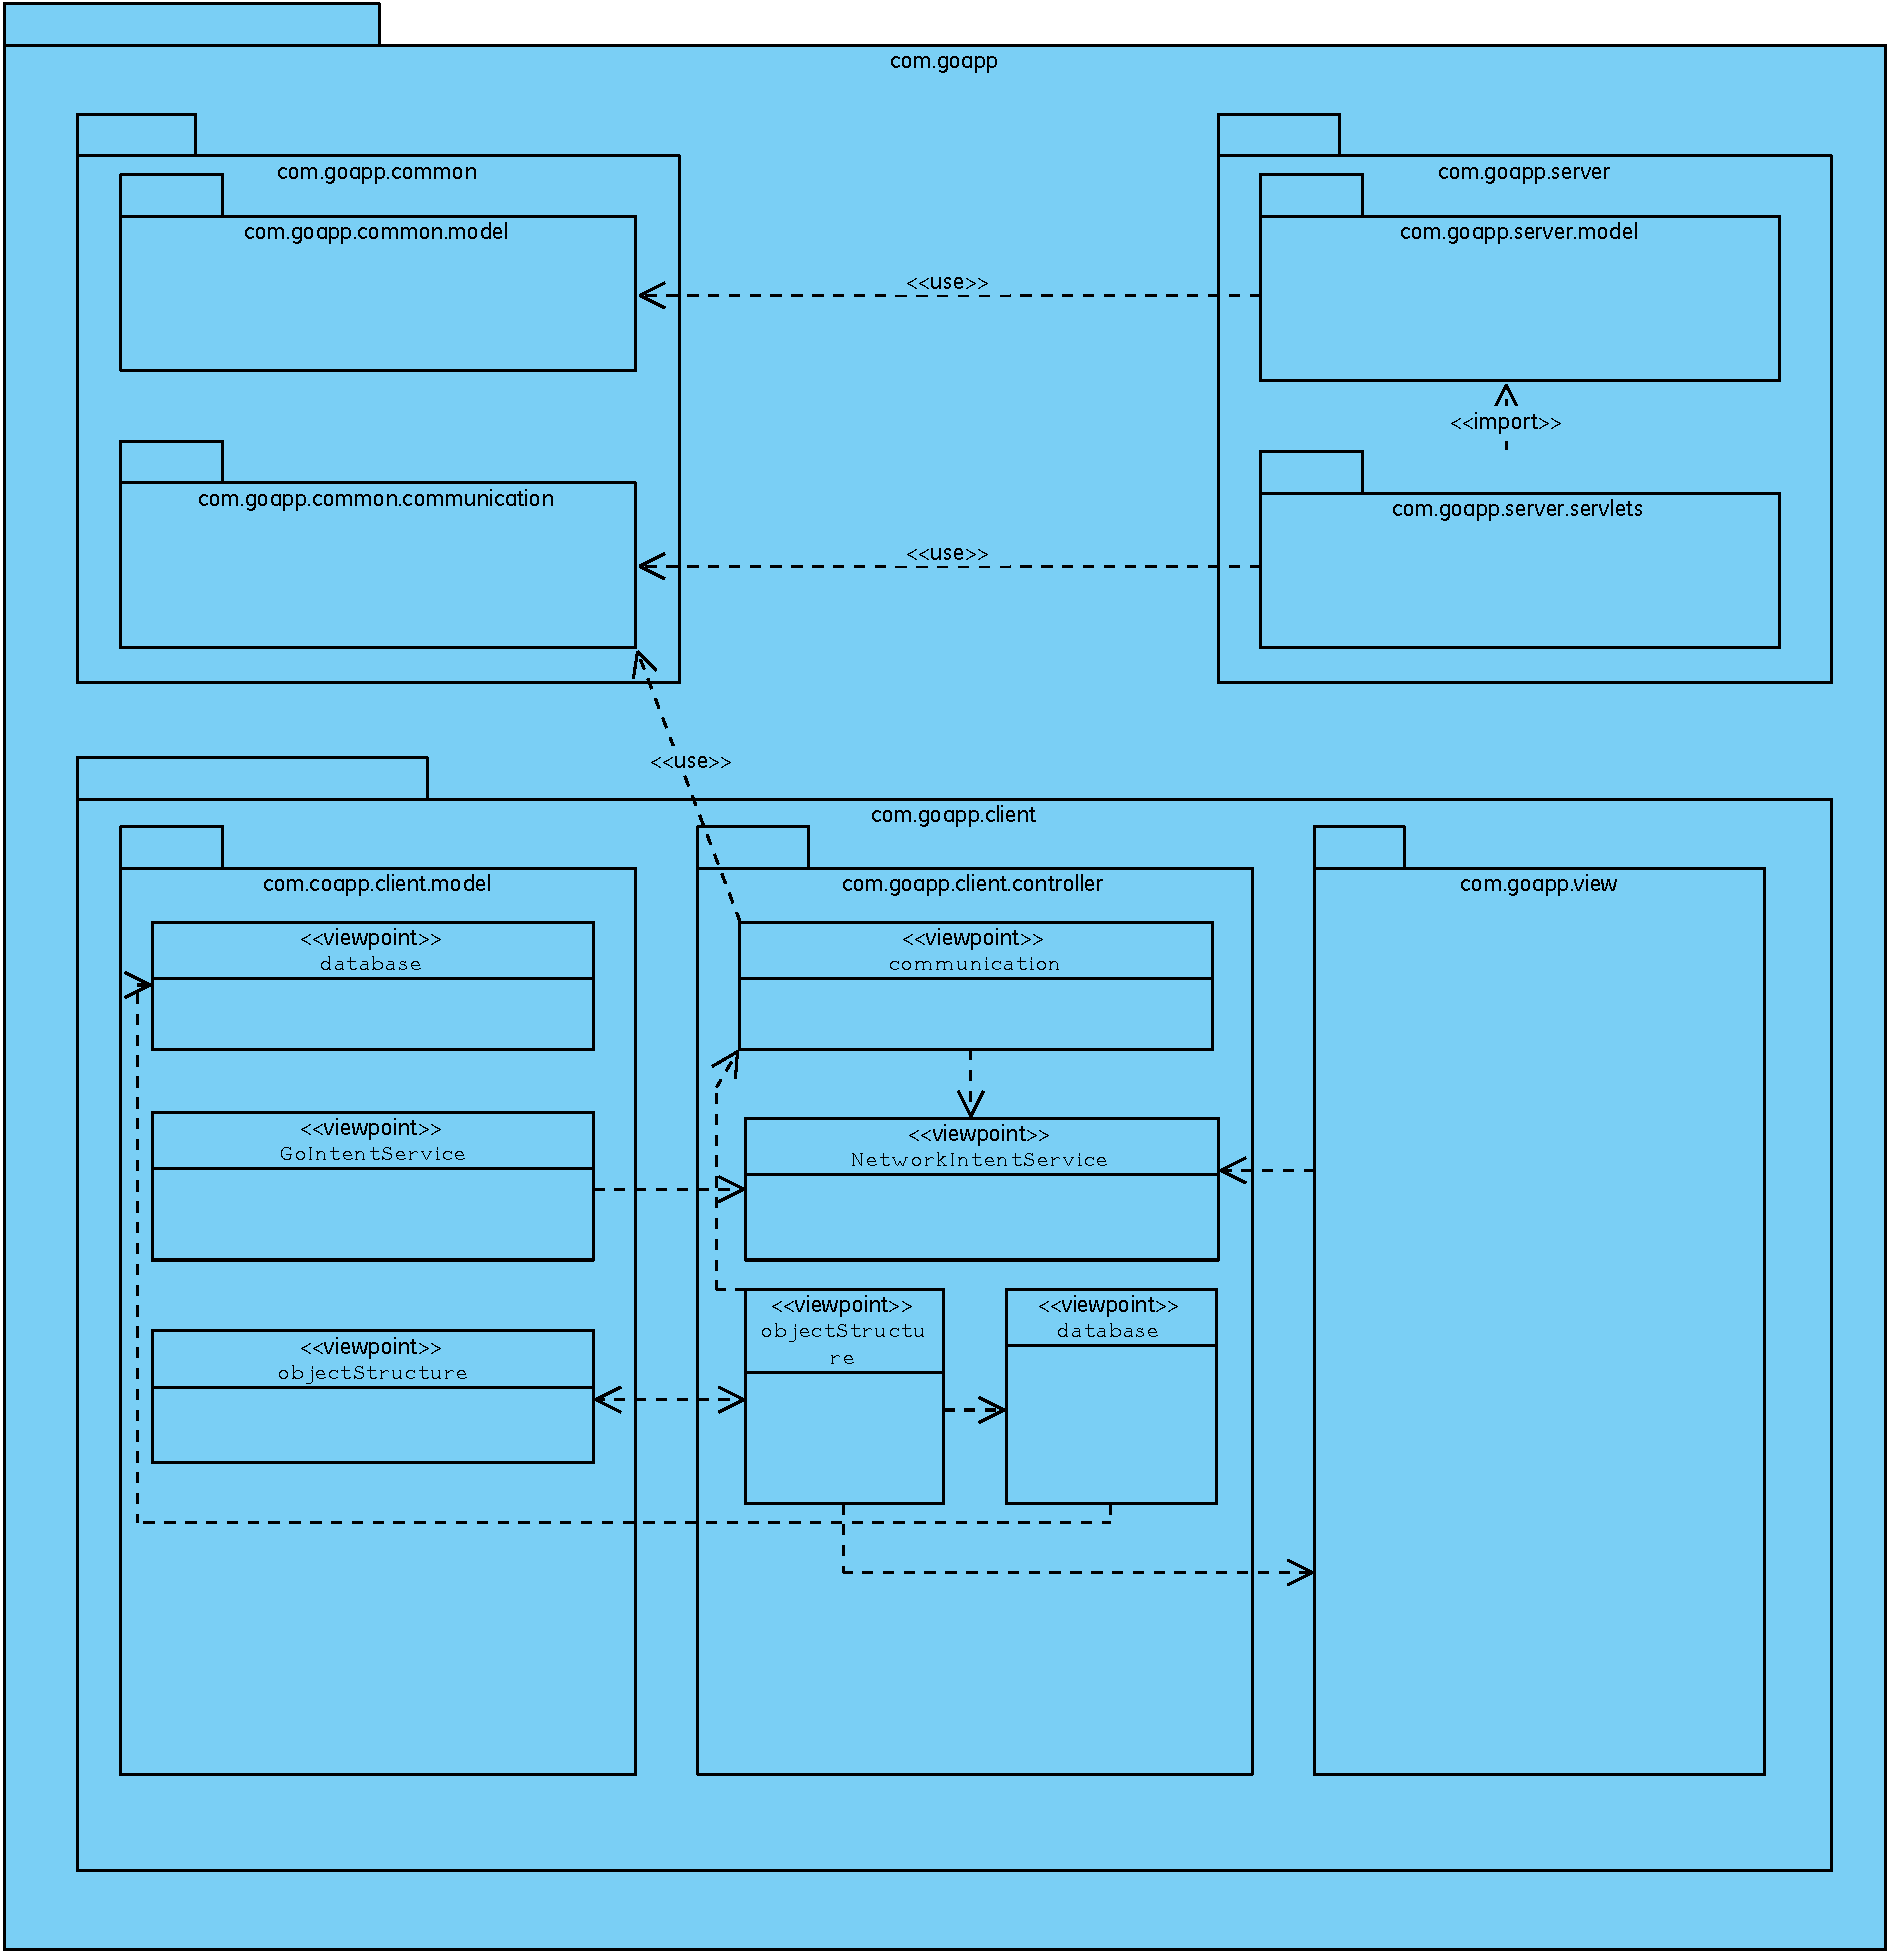
\includegraphics[scale=0.5, trim=2 2 2 2, clip=true]{servergraphs/package-server.pdf}
     \caption{Paketdiagramm Gesamt}
\end{figure}
\clearpage
\subsection{Architekturstil}

\subsubsection{Clientseitig}
--> MVC nicht ganz eindeutig Model und Controler wegen Activities und Fragments überschneiden sich

\subsubsection{Serverseitig}

\subsection{Paketdiagramm}






\newpage
\section{Feinentwurf}
Detaillierte Beschreibung aller Klassen. Das beinhaltet (JavaDoc) Beschreibungen zu allen Methoden, Konstruktoren, Packages und Klassen. Was hier nicht reingehört sind private Felder und Methoden. Das sind Implementierungsdetails.

Identifikation von Entwurfsmustern um Struktur gröber zu beschreiben.

Definition von GroupID, UserId,... was wir alles besprochen haben

\subsection{Clientseitig}
\subsubsection{ClientView}
\begin{enumerate}
	%- hier muss das PDF mit der Gesamtübersicht hin
	\item \textbf{\underline{MainActivity}}
	
	%- hier muss das PDF classcom_1_1example_1_1androidgoapp_1_1androidgoapp_1_1view_1_1_main_activity__inherit__graph.pdf eingebunden werden
	Aufgrund der MVC Struktur der App ist die MainActivity die Hauptactivity des View Teil. Beim Öffnen der App auf dem Client wird diese als erste Activity geöffnet. Sie hat vor allem eine managende Funktion: sie überpfüft ob dieser Client schon registriert ist oder nicht. Sie erbt von der AppCompatActivity und implementiert dementsprechen auch deren Methoden.
	
	\textbf{Methoden}
	\begin{enumerate}
		\item \underline{protected void onCreate(Bundle savedInstanceState)} 
		Erweitert die onCreate Methode der AppCompatActivity indem sie, wenn der Client schon registriert ist, erst an die UsernameActivity weiterleitet. Ist er jedoch schon registriert, so leitet sie direkt an die zuletzt aufgerufene GroupActivity weiter.
		\item \underline{protected void onStart()}
		Erweitert die onStart() Methode der AppCompatActivity %- blabla ich habe keine Ahnung, was die wirklich macht
		\item \underline{protected void onRestart()}
		Erweitert die onRestart() Methode der AppCompatActivity %- blabla ich habe keine Ahnung, was die wirklich macht
		\item \underline{protected void onResume()}
		Erweitert die onResume() Methode der AppCompatActivity %- blabla ich habe keine Ahnung, was die wirklich macht
		\item \underline{protected void onPause()}
		Erweitert die onPause() Methode der AppCompatActivity %- blabla ich habe keine Ahnung, was die wirklich macht
		\item \underline{protected void onStop()}
		Erweitert die onStop() Methode der AppCompatActivity %- blabla ich habe keine Ahnung, was die wirklich macht
		\item \underline{protected void onDestroy()}
		Erweitert die onDesroy() Methode der AppCompatActivity %- blabla ich habe keine Ahnung, was die wirklich macht
	\end{enumerate}
	
	\item \textbf{\underline{UsernameActivity}}
	
	%- hier muss das PDF classcom_1_1example_1_1androidgoapp_1_1androidgoapp_1_1view_1_1_username_activity__inherit__graph.pdf eingebunden werden
	Die UsernameActivity ist für das benennen des Benutzernamens zuständig. Sie wird sowohl zum ersten Start der App von der MainActivity aufgerufen, als auch von von der GroupActivity, wenn der Benutzer auf den Benutzernamen tippt. Sie enthält das UsernameChangeFragment und das UsernameRegistrationFragment. Sie erbt von der AppCompatActivity und implementiert dementsprechen auch deren Methoden.
	
	\textbf{Methoden}
	
	\begin{enumerate}
		\item \underline{protected void onCreate(@Nullable Bundle savedInstanceState)}
		Erweitert die onCreate Methode der AppCompatActivity mit dem laden des UsernameChangeFragments.
	\end{enumerate}
	
	\item \textbf{\underline{UsernameRegistrationFragment}}
	
	%- hier muss das PDF classcom_1_1example_1_1androidgoapp_1_1androidgoapp_1_1view_1_1_username_registration_fragment__inherit__graph.pdf eingebunden werden
	Das UsernameCreateFragment ist dafür zuständig einen neuen User auf dem Server anzulegen. Es wird auf jedem Client in den username\_container der UsernameActivity geladen und somit nur einmalig aufgerufen, bis sich der Benutzer registriert hat. Es legt die erste Ansicht fest, die ein Benutzer sieht, wenn er die App das erste mal öffnet, bzw. wenn er die App öffnet und sich noch nie registriert hat. Es erbt von Fragment und implementiert den View.onClickListener. Dementsprechend implementiert sie auch deren Methoden.
	
	\textbf{Methoden}
	
	\begin{enumerate}
		\item \underline{public View onCreateView(LayoutInflater inflater, ViewGroup container, Bundle savedInstanceState)}
		Erweitert die onCreateView Methode des Fragments mit der gewünschten Ansicht, die der View übergeben wird und fürgt dem OnClickListener den Button hinzu. Diese Methode gibt die aktuelle View zurück.
		\item \underline{public void onClick(View view)}
		Implementiert die onClick Methode des OnClickListeners, so dass beim Klicken auf den Next-Button überprüft wird, ob der gewünschte Benutzername zugelassen ist. In diesem Fall legt er einen neuen User an und leitet an eine leere GroupActivity weiter.
	\end{enumerate}

	\item \textbf{\underline{UsernameChangeFragment}}
		
	%- hier muss das PDF classcom_1_1example_1_1androidgoapp_1_1androidgoapp_1_1view_1_1_username_change_fragment__inherit__graph.pdf eingebunden werden
	Das UsernameChangeFragment ist dafür zuständig den Username zu ändern. Es wird von der UsernameActivity in den username\_container geladen. Es legt die Ansicht fest, die ein Benutzer sieht, wenn er seinen Benutzernamen ändern möchte. Es erbt von Fragment und implementiert den View.onClickListener. Dementsprechend implementiert es auch deren Methoden.
	
	\textbf{Methoden}
	
	\begin{enumerate}
		\item \underline{public View onCreateView(LayoutInflater inflater, ViewGroup container, Bundle savedInstanceState)}
		Erweitert die onCreateView Methode des Fragments mit der gewünschten Ansicht, die der View übergeben wird und fügt dem OnClickListener den Button hinzu, wenn der Benutzer die App nicht zum ersten Mal öffnet. In diesem Fall lädt es das UsernameRegistrationFragment in den username\_container der UsernameActivity. Diese Methode gibt die aktuelle View zurück.
		\item \underline{public void onClick(View view)}
		Implementiert die onClick Methode des OnClickListeners, so dass beim Klick auf dem Next-Button überprüft wird, ob der gewünschte neue Benutzername zugelassen ist. In diesem Fall ändert er diesen und leitet an die zuletzt aufgerufene GroupActivity weiter.
	\end{enumerate}
	
	\item \textbf{\underline{GroupActivity}}
	
	%- hier muss das PDF classcom_1_1example_1_1androidgoapp_1_1androidgoapp_1_1view_1_1_group_activity__inherit__graph.pdf eingebunden werden
	GroupActivity ist für das Management der Gruppe zuständig. Sie ist die Activity, die die meiste Zeit geöffnet ist. Von allen anderen Activitys aus kann sie aus geöffnet werden. Sie enthält das Group
	
	\textbf{Methoden}
	
	\begin{enumerate}
		\item \underline{}
		
	\end{enumerate}
	
	\item \textbf{\underline{GroupMapFragment}}
	
	%- hier muss das PDF classcom_1_1example_1_1androidgoapp_1_1androidgoapp_1_1view_1_1_group_map_fragment__inherit__graph.pdf eingebunden werden
	Das GroupMapFragment ist dafür zuständig, die Map-Ansicht anzuzeigen. Es wird von der GroupActivity in den group\_container geladen, immer dann wenn eine Gruppe aufgerufen wird. Es legt die Map-Ansicht einer Gruppe fest. Es erbt von Fragment und implementiert den View.onClickListener. Dementsprechend implementiert es auch deren Methoden.
	
	\textbf{Methoden}	
	\begin{enumerate}
		\item \underline{public View onCreateView(LayoutInflater inflater, ViewGroup container, Bundle savedInstanceState)}
		Erweitert die onCreateView Methode des Fragments mit der gewünschten Ansicht, die der View übergeben wird und fügt dem OnClickListener die Button hinzu, wenn der Benutzer den Go-Button nicht gedrückt hat. In diesem Fall lädt es das GroupMapFragmentGo in den group\_container der GroupActivity. Diese Methode gibt die aktuelle View zurück.
		\item \underline{public void onClick(View view)}
		Implementiert die onClick Methode des OnClickListeners, so dass er beim Klick auf den Gruppennamen das GroupMembersFragment in den group\_container der GroupActivity lädt, beim Klick auf das Datum, wenn man Gruppenadministrator ist, das GroupAppointmentFragment in den group\_container der GroupActivity lädt und beim Klick auf den Go-Button das GroupActivityGoFragment in den group\_container der GroupActivity lädt.	
	\end{enumerate}
	
	\item \textbf{\underline{DatePickerFragment}}
	
	%- hier muss das PDF classcom_1_1example_1_1androidgoapp_1_1androidgoapp_1_1view_1_1_date_picker_fragment__inherit__graph.pdf eingebunden werden
	%- text
	
	\textbf{Methoden}
	\begin{enumerate}
		\item \underline{}
		
	\end{enumerate}
	
	\item \textbf{\underline{GroupAppointmentFragment}}
	%- hier muss das PDF classcom_1_1example_1_1androidgoapp_1_1androidgoapp_1_1view_1_1_group_appointment_fragment__inherit__graph.pdf eingebunden werden
	%- text
	
	\textbf{Methoden}
	\begin{enumerate}
		\item \underline{}
		
	\end{enumerate}

	\item \textbf{\underline{GroupMapFragmentGo}}

	%- hier muss das PDF classcom_1_1example_1_1androidgoapp_1_1androidgoapp_1_1view_1_1_group_map_fragment_go__inherit__graph.pdf eingebunden werden
	%- text
	
	\textbf{Methoden}
	\begin{enumerate}
		\item \underline{}
		
	\end{enumerate}

	\item \textbf{\underline{GroupMembersFragment}}
	
	%- hier muss das PDF classcom_1_1example_1_1androidgoapp_1_1androidgoapp_1_1view_1_1_group_members_fragment__inherit__graph.pdf eingebunden werden
	%- text
	
	\textbf{Methoden}
	\begin{enumerate}
		\item \underline{}
		
	\end{enumerate}

	\item \textbf{\underline{GroupnameActivity}}
	
	%- hier muss das PDF classcom_1_1example_1_1androidgoapp_1_1androidgoapp_1_1view_1_1_groupname_activity__inherit__graph.pdf eingebunden werden
	%- text
	
	\textbf{Methoden}
	\begin{enumerate}
		\item \underline{}
		
	\end{enumerate}
	
	\item \textbf{\underline{GroupnameChangeFragment}}
	
	%- hier muss das PDF classcom_1_1example_1_1androidgoapp_1_1androidgoapp_1_1view_1_1_groupname_change_fragment__inherit__graph.pdf eingebunden werden
	%- text
	
	\textbf{Methoden}	
	\begin{enumerate}
		\item \underline{}
		
	\end{enumerate}

	\item \textbf{\underline{GroupnameCreateFragment}}
	
	%- hier muss das PDF classcom_1_1example_1_1androidgoapp_1_1androidgoapp_1_1view_1_1_groupname_create_fragment__inherit__graph.pdf eingebunden werden
	%- text
	
	\textbf{Methoden}
	
	\begin{enumerate}
		\item \underline{}
		
	\end{enumerate}
	\item \textbf{\underline{MemberAdapter}}
	
	%- hier muss das PDF classcom_1_1example_1_1androidgoapp_1_1androidgoapp_1_1view_1_1_member_adapter__inherit__graph.pdf eingebunden werden
	%- text
	
	\textbf{Methoden}
	\begin{enumerate}
		\item \underline{}
		
	\end{enumerate}
	\item \textbf{\underline{TimePickerFragment}}
	
	%- hier muss das PDF classcom_1_1example_1_1androidgoapp_1_1androidgoapp_1_1view_1_1_time_picker_fragment__inherit__graph.pdf eingebunden werden
	%- text
	
	\textbf{Methoden}
	\begin{enumerate}
		\item \underline{}
		
	\end{enumerate}
\end{enumerate}
\subsubsection{ClientModel}

\textbf{GoIntentService}
\begin{figure}[H]
	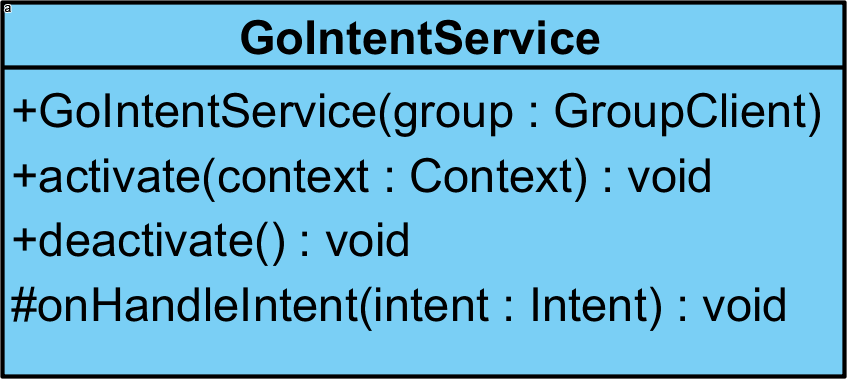
\includegraphics[scale = .3]{res/umlClasses/GoIntentService.png}
	\centering	
\end{figure}
Der GokIntentService kümmert sich um Netzwerkanfragen die den GoStatus, also Anfragen in regelmäßigen Zeitintervallen an den Server sendet und Koordinaten übermittelt. Dieser Service läuft im Hintergrund ab, um die Benutzeroberfläche nicht zu behindern.
\begin{enumerate}
	\item public GoIntentService(group: Group)
		Konstruktor für den IntentService.
	\item public activate(context: Context):void
		GoIntetnService wird aktiviert, wenn der GoStatus aktiviert wurde.
	\item public deactivate():void
		GoIntentService wird deaktiviert, wenn der GoStatus deaktiviert wurde.
	\item protected onHandleIntent(intent: Intent): void
		Für jede Netzwerkanfrage wird ein neuer Thread gestartet und es wird verhindert, dass Anfragen beim Drehen des Bildschirms verloren gehen.
\end{enumerate}

\paragraph{Database}
\begin{figure}[H]
	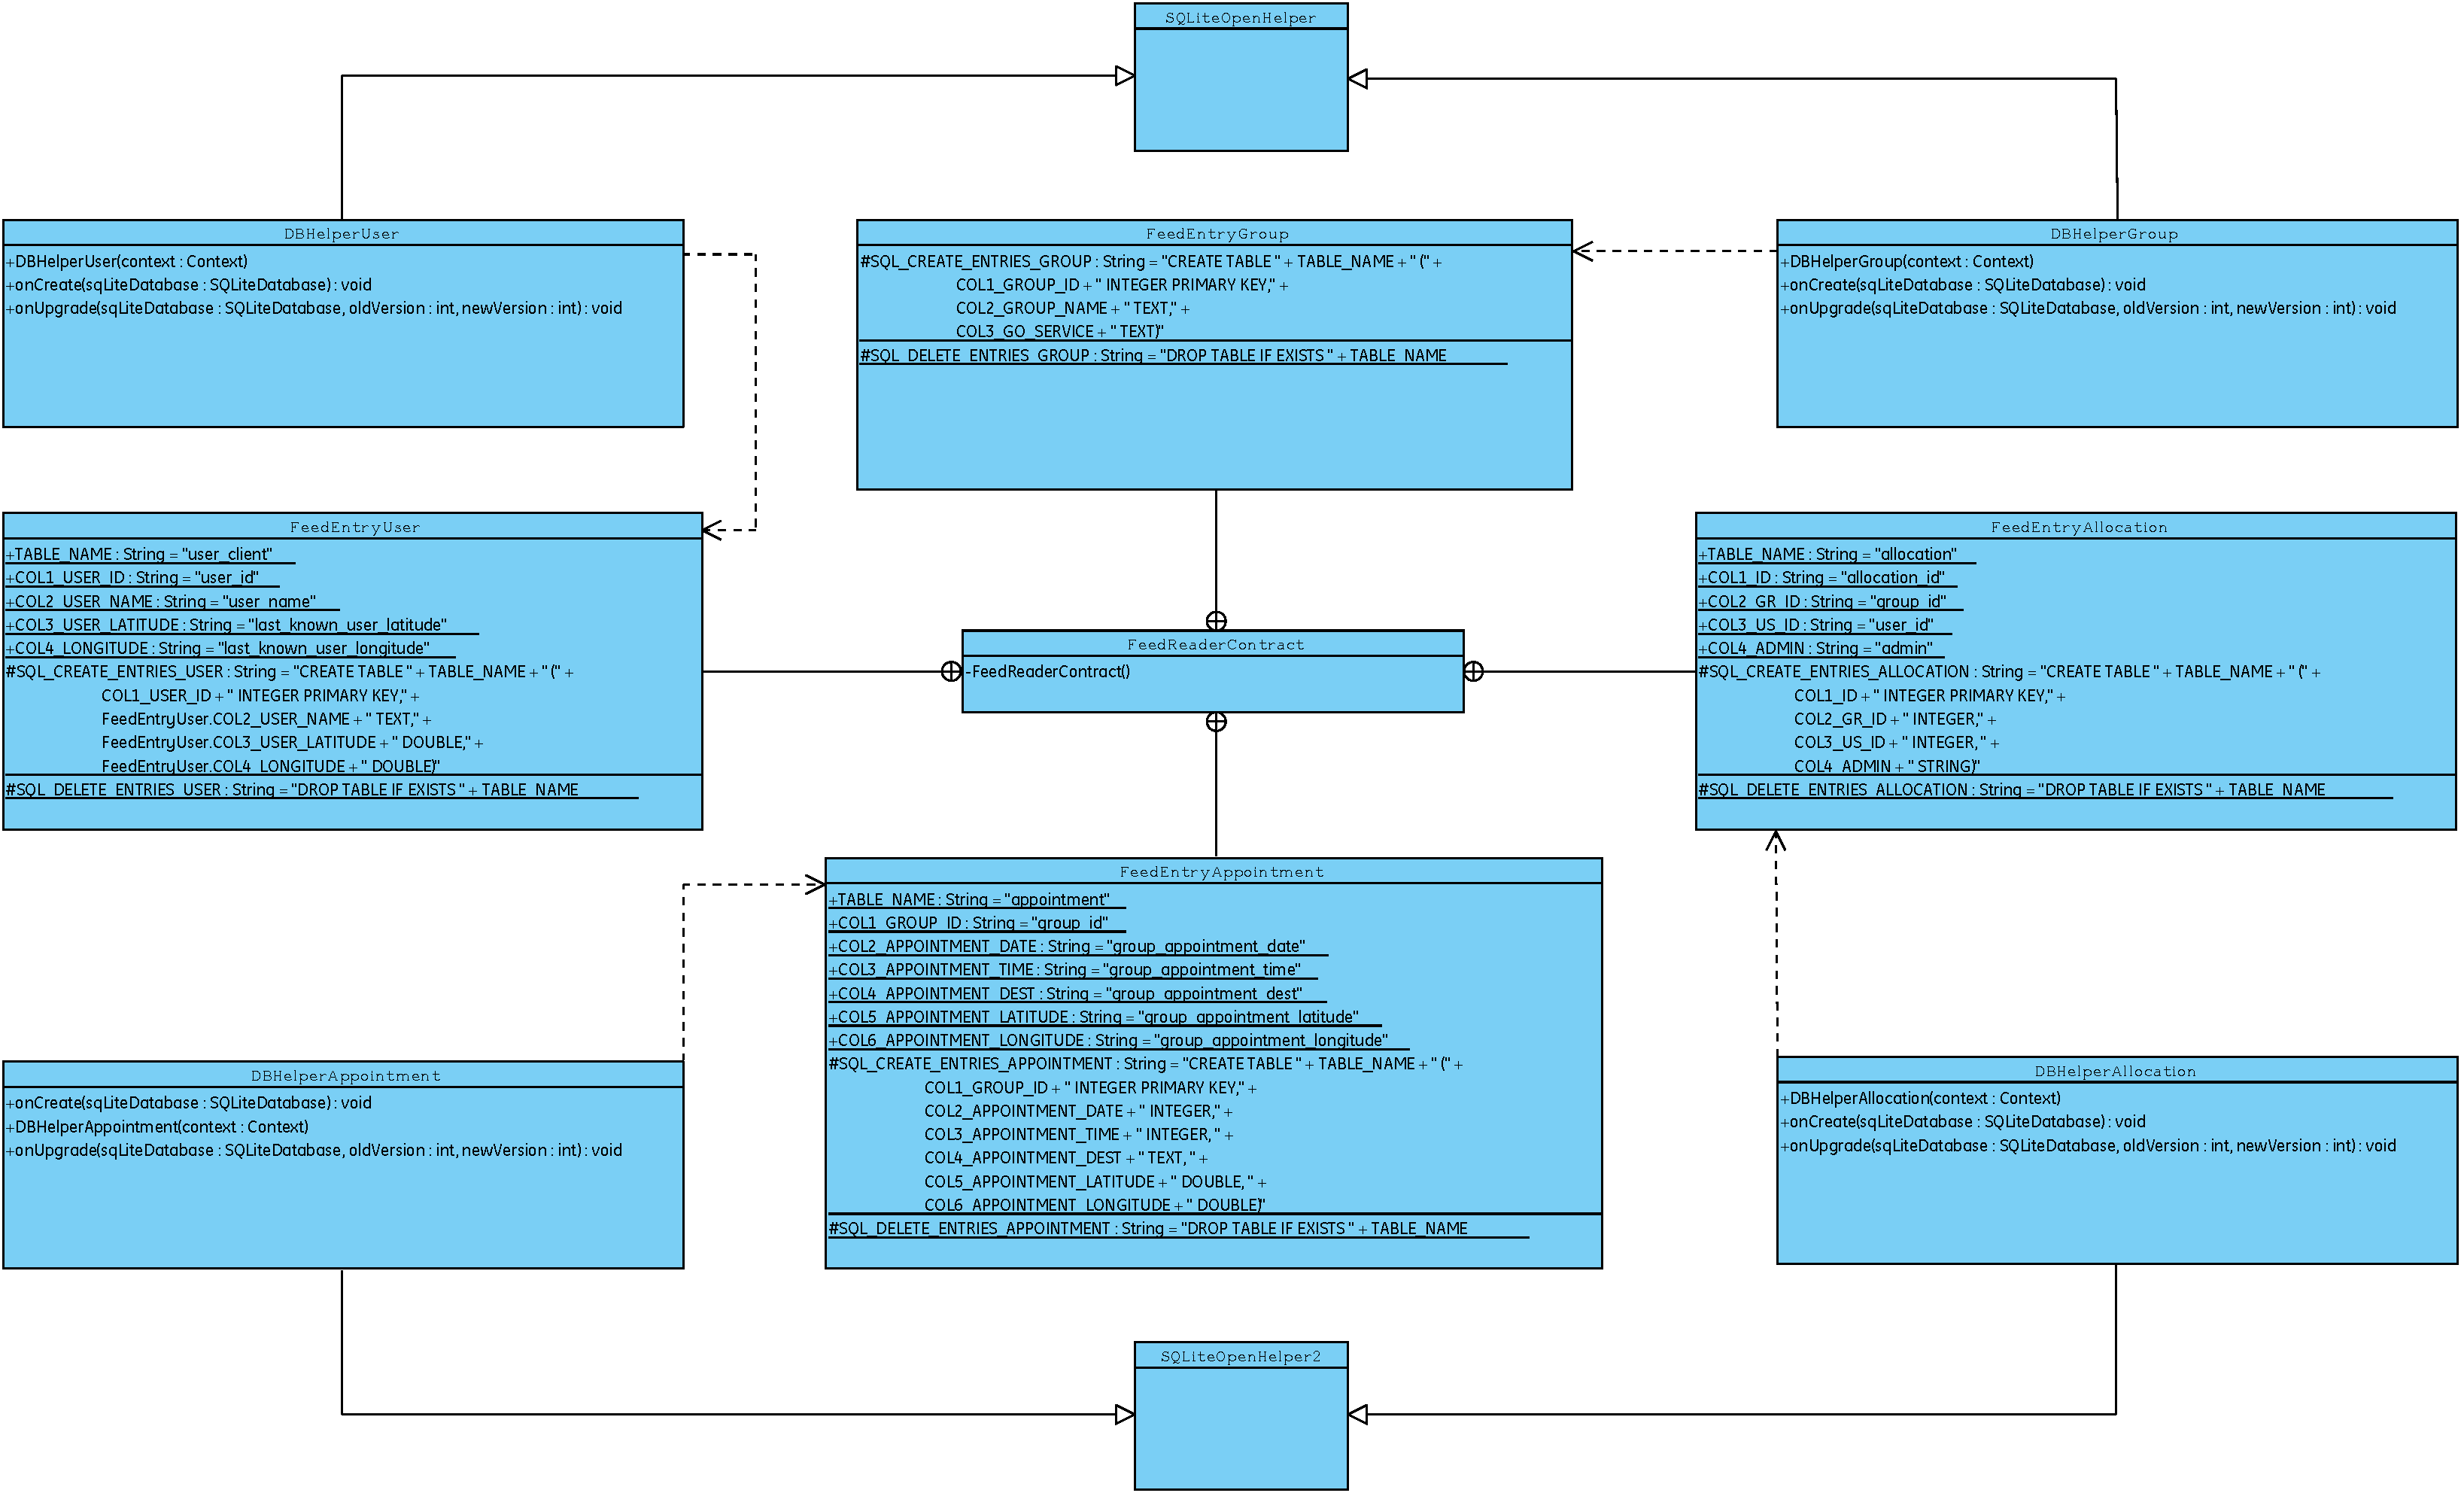
\includegraphics[scale = .3]{res/umlDiagramms/modelClientDatabase.pdf}
	\centering	
\end{figure}

\textbf{DBHelper}\\
Die vier nachfolgenden DBHelper erben ihren Konstruktor und ihre Methoden von SQLiteOpenHelper. 
\begin{enumerate}
	\item public DBHelperGroup(context: Context)\\
		Der Konstruktor definiert dabei den Namen und die Versionsnummer der Datenbank.
	\item public onCreate(sqLiteDatabase: SQLiteDatabase)\\
		Die SQLiteDatenbank wird mit den in FeedReaderEntry definierten Spalten aufgebaut, wenn sie das erste Mal aufgerufen wird.
	\item public onUpgrade(sqLiteDatabase: SQLiteDatabase, oldVersion: int, newVersion: int)\\
		Diese Methode wird verwendet, wenn man die Datenbank verändert hat. Dieser wird dann eine neue Versionsnummer zugeteilt.	
\end{enumerate}
\begin{figure}[H]
	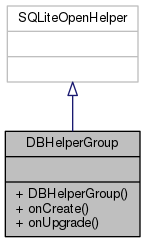
\includegraphics[scale = .5]{res/umlClasses/DBHelperGroup.png}
	\centering	
\end{figure}

\begin{figure}[H]
	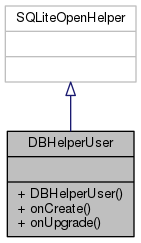
\includegraphics[scale = .5]{res/umlClasses/DBHelperUser.png}
	\centering
\end{figure}

\begin{figure}[H]
	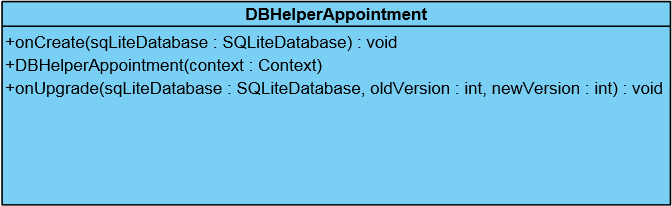
\includegraphics[scale = .58]{res/umlClasses/DBHelperAppointment.png}
	\centering
\end{figure}

\begin{figure}[H]
	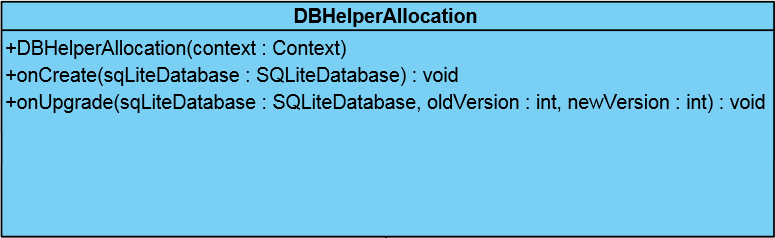
\includegraphics[scale = .5]{res/umlClasses/DBHelperAllocation.png}
	\centering
\end{figure}


\textbf{FeedReaderContract}
\begin{figure}[H]
	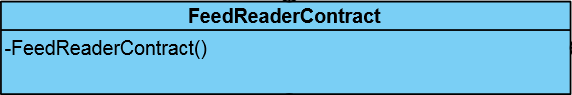
\includegraphics[scale = .5]{res/umlClasses/FeedReaderContract.png}
	\centering
\end{figure}
Die FeedReaderContract Klasse definiert in statischen Innenklassen wie die Tabellen der Datenbank aufgebaut sind. Jede der nachfolgenden FeedEntry Klassen implementiert dabei das Interface BaseColumns.

\begin{enumerate}
	\item public static final CREATE ENTRIES:String\\
		Legt die Spalten wenn die Tabelle generiert wird in genau dieser Reihenfolge an.
	\item public static final DELETE ENTRIES:Strning\\
		Löscht die zuvor definierten Spalteneinträge.
\end{enumerate}

\textbf{FeedEntyGroup}
\begin{figure}[H]
	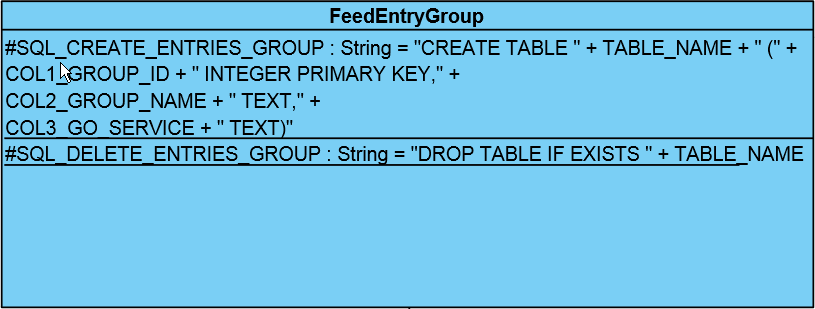
\includegraphics[scale = .5]{res/umlClasses/FeedEntryGroup.png}
	\centering
\end{figure}
Die Innenklasse FeedEntryGroup definiert den Namen und die Spalten der Tabelle, welche die Gruppen auf dem Client speichert. 
Dabei steht in der ersten Spalte die eindeutige Gruppen ID (welche die Zeilen eindeutig unterscheidbar macht), in der zweiten Spalte der eindeutige Gruppenname und in der dritten Spalte, ob der GoService des aktuellen Benutzers für diese Gruppe aktiviert oder deaktiviert ist.
Wenn eine Gruppe gelöscht wird, dann wird auch ihr Eintrag in der Datenbank gelöscht.

\textbf{FeedEntyUser}
\begin{figure}[H]
	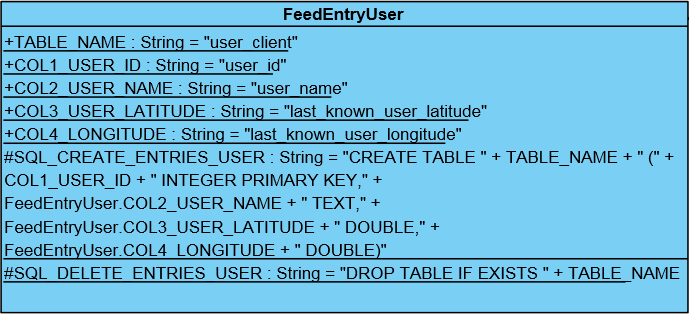
\includegraphics[scale = .6]{res/umlClasses/FeedEntryUser.png}
	\centering
\end{figure}
Die Innenklasse FeedEntryUser definiert den Namen und die Spalten der Tabelle, welche die Benutzer auf dem Client speichert. 
Dabei steht in der ersten Spalte die eindeutige Benutzer ID (welche die Zeilen eindeutig unterscheidbar macht), in der zweiten Spalte der Benutzername und in der dritten und vierten Spalte steht je ein Wert der zuletzt bekannten Gps Daten des jeweiligen Nutzers. 
Es werden nur Benutzer gespeichert mit denen der aktuelle Benutzer in mindestens einer gemeinsamen Gruppe ist.

\textbf{FeedEntyAppointment}
\begin{figure}[H]
	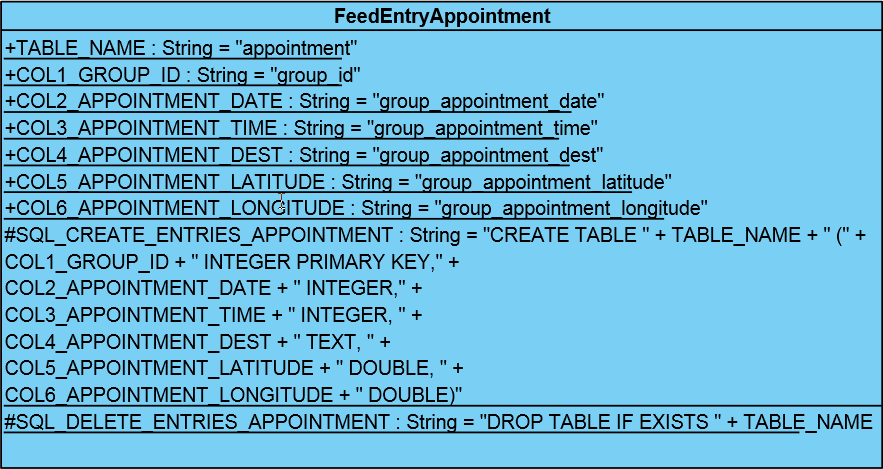
\includegraphics[scale = .5]{res/umlClasses/FeedEntryAppointment.png}
	\centering
\end{figure}
Die Innenklasse FeedEntryAppointment definiert den Namen und die Spalten der Tabelle, welche die Treffpunkte zu jeder Gruppe speichert. Jede Gruppe hat dabei nur eine Zeile, welche den Treffpunkt definiert. 
Dabei steht in der ersten Spalte die Gruppen id (welche die Zeilen eindeutig unterscheidbar macht), in der zweiten Spalte steht das Datum und in der dritten die Uhrzeit des Treffpunktes. In der vierten Spalte steht der Name des Zielortes und in der fünften und sechsten steht jeweils ein Wert der Gps Daten des Zielortes. 
Wenn sich der Treffpunkt der Gruppe ändert, dann werden die Werte des alten Treffpunktes überschrieben.
Sollte die die Gruppe des dazugehörigen Treffpunktes gelöscht werden, dann wird auch der Eintrag in dieser Tabelle gelöscht.

\textbf{FeedEntyAllocation}
\begin{figure}[H]
	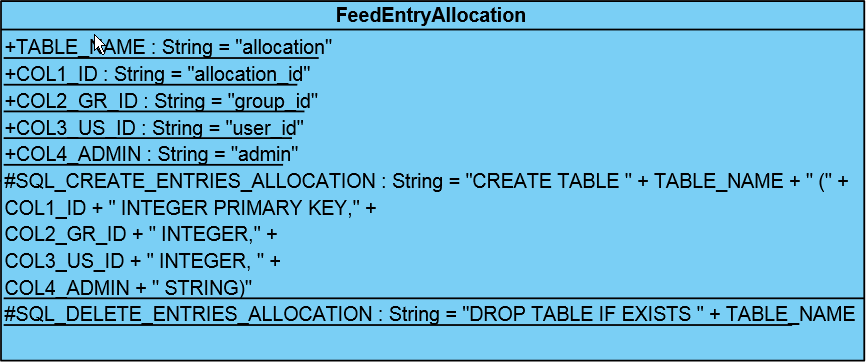
\includegraphics[scale = .5]{res/umlClasses/FeedEntryAllocation.png}
	\centering
\end{figure}
Die Innenklasse FeedEntryAllocation definiert den Namen und die Spalten der Tabelle, welche die jeweiligen Mitglieder jeder Gruppe speichert, in der der aktuelle Benutzer Mitglied ist. Zu jedem Mitglied wird vermerkt, ob dieses Administratorrechte hat.
Dabei steht in der ersten Spalte die Allocation id (welche die Zeilen eindeutig unterscheidbar macht und automatisch hochgezählt), in der zweiten Spalte steht die Gruppen id, in der dritten Spalte die Benutzer id und in der vierten Spalte, ob dieser Benutzer Gruppenadministrator ist oder nicht. 
Gruppen id wird für jedes Gruppenmitglied vermerkt, also kommt mehrmals vor, sobald mehr als ein Benutzer Mitglied dieser Gruppe ist.


\paragraph{ObjectStructure}

\begin{figure}[H]
	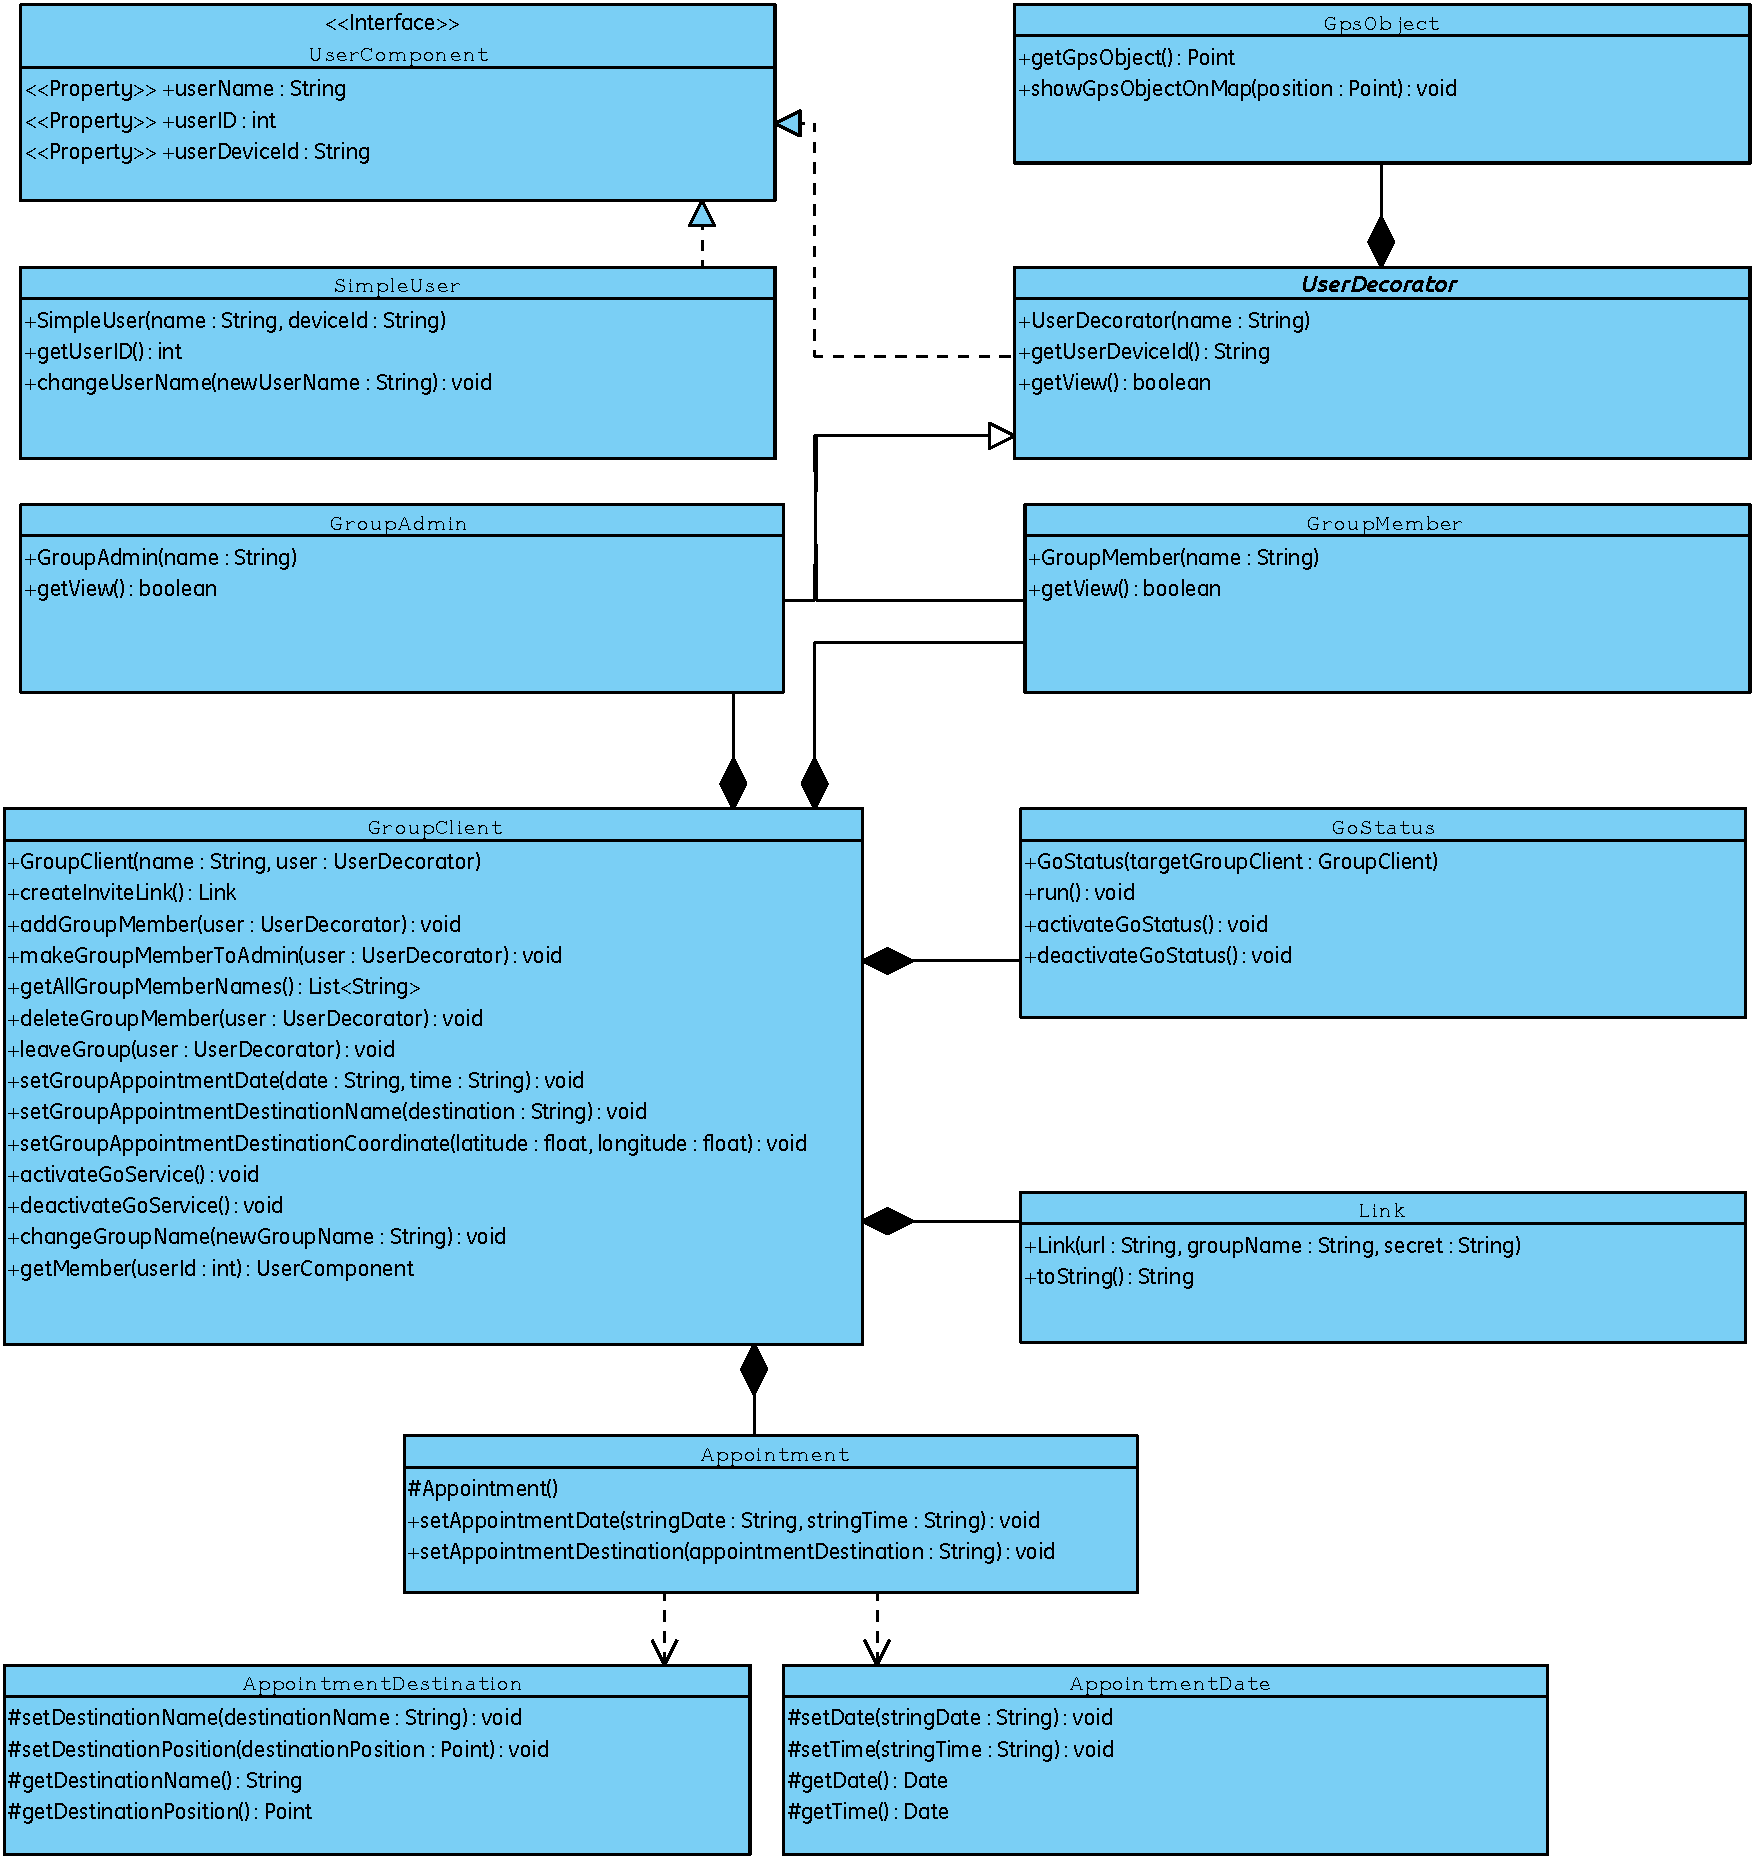
\includegraphics[scale = .5]{res/umlDiagramms/modelClientObjectStructure.pdf}
	\centering	
\end{figure}

\textbf{GroupClient}
\begin{figure}[H]
	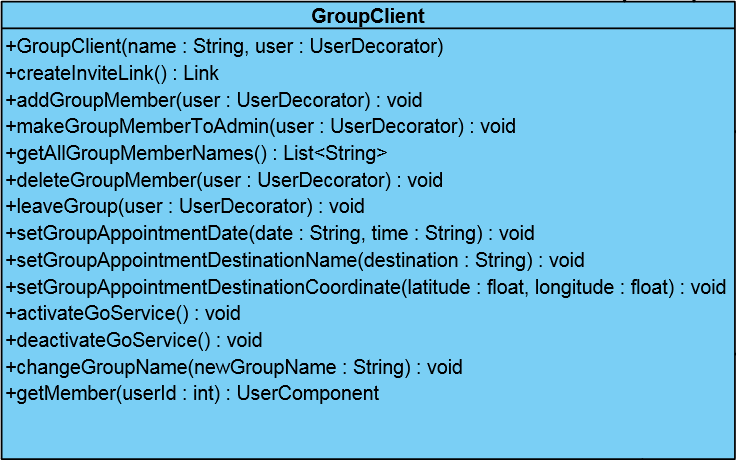
\includegraphics[scale = .5]{res/umlClasses/GroupClient.png}
	\centering
\end{figure}
Die Klasse GroupClient definiert wie eine Gruppe auf dem Client aufgebaut ist und welche Funktionalität ihr zur Verfügung steht.
\begin{enumerate}
	\item public GroupClient(name: String, user: UserDecorator)\\
		Konstruktor der einer neuen Gruppe einen eindeutigen Gruppennamen zuweist und den Ersteller als Gruppenadministrator festlegt.
	\item public createInviteLink():Link\\
		Um ein Gruppenmitglied hinzuzufügen, muss dieses über einen eindeutigen Link beitreten. Wird der Link ausgeführt wird man entweder zu GoApp weitergeleitet (hat App bereits installiert) oder wird dazu aufgefordert diese zu installieren. Der Link ist nicht mehr gültig sobald das Mitglied hinzugefügt wurde. Man muss Administrator sein um diese Funktion verwenden zu können.
	\item public addGroupMember(user: UserDecorator)\\
		Ein Mitglied wird der Gruppe hinzugefügt.
	\item public makeGroupMemberToAdmin(user: UserDecorator)\\
		Ein Gruppenmitglied wird vom Administrator zum Gruppenadministrator gemacht.
	\item public getAllGroupMemberNames():List<String>\\
		Alle Namen der Mitglieder einer Gruppe werden zurückgegeben.
	\item public deleteGroupMember(user:UserDecorator)\\
		Ein Gruppenmitglied wird aus der Gruppe durch den Administrator entfernt.
	\item public leaveGroup(user:UserDecorator)\\
		Ein Mitglied verlässt die Gruppe.
	\item public activateGoService()\\
		Der aktuelle Benutzer aktiviert seinen GoStatus und übermittelt seine GPS Daten an die Gruppe (GPS muss eingeschalten sein).
	\item public deactivateGoService()\\
		Der aktuelle Benutzer deaktiviert seinen GoStatus und wird nicht mehr verfolgt.
	\item public changeGroupName(newGroupName:String)\\
		Der Gruppenadministrator benennt die Gruppe zu einem anderen eindeutigen Namen um.
	\item public getGroupID():int \\
		Die Gruppen Id wird zurückgegeben
	\item public getGroupName():String\\
		Der Gruppenname wird zurückgegeben 
	\item public getGoStatus():GoStatus \\
		Der GoStatus wird zurückgegeben
	\item public getAppointment():Appointment \\
		Das Appointment wird zurückgegeben
	\item public getMember(userId: int):UserComponent \\
		Der Typ des aktuellen Benutzers einer Gruppe (Gruppenmitglied oder Administrator)wird zurückgegeben, um die Ansicht der Gruppe auf seine ihm zugänglichen Funktionen zu beschränken/ erweitern.
\end{enumerate}

\textbf{UserComponent}
\begin{figure}[H]
	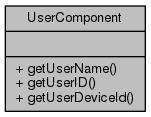
\includegraphics[scale = .5]{res/umlClasses/UserComponent.png}
	\centering
\end{figure}
Dieses Interface ist die erste Komponente des Decorator pattern und definiert grundlegende Funktionen des Benutzers die jederzeit aufgerufen werden können. 

Mit getUserId() kann der Benutzer von anderen Gruppenmitgliedern unterschieden werden, da der Benutzername nicht eindeutig sein muss, die Id aber schon.
Mit getUserDeviceId() kann der Benutzer auf dem Server angelegt werden. Jede Gerätenummer kann nur einmal auf dem Server vorkommen, um Missbrauch der GoApp vorzubeugen.
\begin{enumerate}
	\item public getUserName():String\\
		Benutzername des aktuellen Benutzers kann in der GoApp visualisiert werden.
	\item public getUserID():int\\
		Mit der Benutzer Id kann sich der aktuelle Benutzer unter den anderen Gruppenmitglieder identifizieren.
	\item public getUserDeviceID():String\\
		Die Device Id wird auf dem Server zusammen mit den anderen zwei Werten gespeichert, um einem Endgerät nur einen Benutzer zu erlauben, um Missbrauch zu vermeiden.
\end{enumerate}

\textbf{SimpleUser}
\begin{figure}[H]
	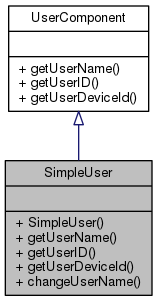
\includegraphics[scale = .5]{res/umlClasses/SimpleUser.png}
	\centering
\end{figure}
Die SimpleUser Klasse implementiert das UserComponent Interface. Der Benutzer ist ein SimpleUser Objekt, wenn er nicht in der Gruppenansicht ist und so weder einem Gruppenadministrator noch einem Gruppenmitglied entspricht.
\begin{enumerate}
	\item public getUserName():String\\
		Siehe UserComponent.
	\item public getUserID():int\\
		Siehe UserComponent.
	\item public getUserDeviceID():String\\
		Siehe UserComponent.
	\item public changeUserName(newUserName: String)\\
	Der aktuelle Benutzer kann seinen Benutzernamen nachträglich ändern.
\end{enumerate}

\textbf{UserDecorator}
\begin{figure}[H]
	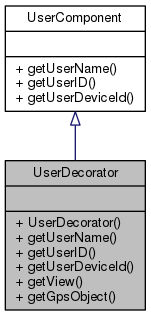
\includegraphics[scale = .5]{res/umlClasses/UserDecorator.png}
	\centering
\end{figure}
Die UserDecorator Klasse ist eine abstrakte Klasse, die wie SimpleUser das UserComponent Interface implementiert. 
\begin{enumerate}
	\item public getUserName():String\\
		Siehe UserComponent.
	\item public getUserID():int\\
		Siehe UserComponent.
	\item public getUserDeviceID():String\\
		Siehe UserComponent.
	\item public getView():boolean\\
		Mit dieser Methode wird bestimmt welche Gruppenansicht der aktuelle Benutzer sieht (die für ein Gruppenmitglied oder die für einen Gruppenadministrator mit zusätzlichen Funktionen).
	\item public getGpsObject():GpsObject\\
		Die Gps Daten des aktuellen Benutzers werden zurück gegeben.
\end{enumerate}

\textbf{GroupAdmin}
\begin{figure}[H]
	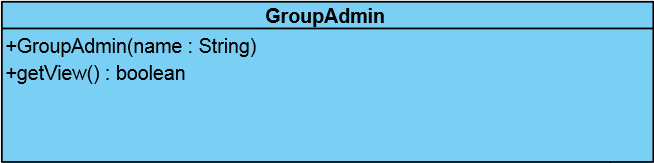
\includegraphics[scale = .5]{res/umlClasses/GroupAdmin.png}
	\centering
\end{figure}
Der Gruppenadministrator unterscheidet sich vom Gruppenmitglied in sofern, dass ihm weitaus mehr Funktionen zur Verfügung stehen, wie Mitglieder hinzufügen/ entfernen und Treffpunkte festlegen.
\begin{enumerate}
	\item public GroupAdmin(name: String)\\
		Konstruktor für einen Gruppenadministrator.
	\item public getView():boolean\\
		Siehe UserDecorator.
\end{enumerate}

\textbf{GroupMember}
\begin{figure}[H]
	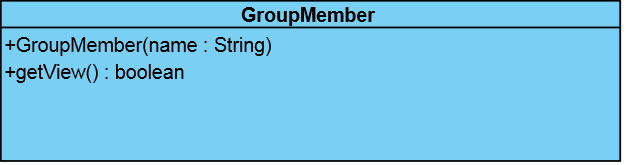
\includegraphics[scale = .5]{res/umlClasses/GroupMember.png}
	\centering
\end{figure}
Das Gruppenmitglied unterscheidet sich vom Gruppenadministrator in sofern, dass ihm die Gruppe betreffend kaum Funktionen zur Verfügung stehen.  
\begin{enumerate}
	\item public GroupMember(name: String)\\
		Konstruktor für einen Gruppenmitglied.
	\item public getView():boolean\\
		Siehe UserDecorator.
\end{enumerate}

\textbf{GoStatus}
\begin{figure}[H]
	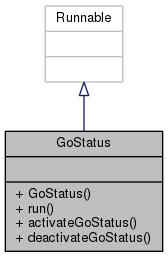
\includegraphics[scale = .5]{res/umlClasses/GoStatus.png}
	\centering
\end{figure}
Der GoStatus bestimmt darüber in welchen Abständen die Position des aktuellen Benutzers an die anderen Gruppenmitglieder übermittelt wird.
\begin{enumerate}
	\item public GoStatus(targetGroupClient: GroupClient)\\
		Konstruktor für den GoStatus wird für jede Gruppe für den aktuellen Benutzer definiert.
	\item public run()\\
		Periodisch bei aktivierten GoStatus der Standort an die Gruppenmitglieder weitergeleitet.
	\item public activateGoStatus()\\
		GoStatus und Gps Tracking aktivieren.
	\item public deactivateGoStatus()\\
		Gps Tracking deaktivieren.
\end{enumerate}

\textbf{Link}
\begin{figure}[H]
	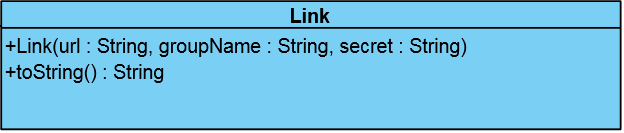
\includegraphics[scale = .5]{res/umlClasses/Link.png}
	\centering
\end{figure}
Mit dem Link kann man andere Mitglieder 
\begin{enumerate}
	\item public Link(url: String, groupName: String , secret: String)\\
		Konstruktor für einen Link. Ein Gruppenlink besteht aus den gelisteten drei Komponenten. Durch den Gruppennamen lässt sich das Mitglied welches den Link betätigt zu derjenigen Gruppe hinzufügen und das sercret verhindert, dass der Link leicht regenerierbar ist.
	\item public toString():String\\
		Der Link wird wieder in seine einzelne Komponenten sortiert.
\end{enumerate}

\textbf{GpsObject}
\begin{figure}[H]
	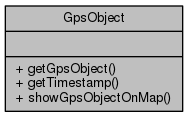
\includegraphics[scale = .5]{res/umlClasses/GpsObject.png}
	\centering
\end{figure}
Das GpsObject gibt an in welcher Form die Gps Daten übermittelt werden.
\begin{enumerate}
	\item public getGpsObject():Point\\
		Der Konstruktor für das GpsObject definiert ein neuen Point der aus einem Längen und einem Breitengrad besteht. 
	\item public getTimestamp():String \\
		Timestamp gibt zurück, wie alt der zuletzt ermittelte Standort ist.
\end{enumerate}

\textbf{Appointment}
\begin{figure}[H]
	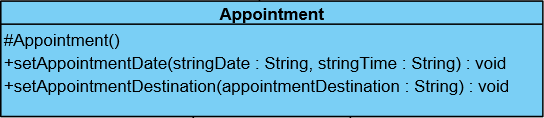
\includegraphics[scale = .6]{res/umlClasses/Appointment.png}
	\centering
\end{figure}
Appointment fasst alle Informationen zusammen die es über den Treffpunkt zu speichern gibt.
\begin{enumerate}
	\item protected Appointment()\\	
		Konstruktor für ein Appointment welches beim Erstellen einer Gruppe default Werte für Datum, Uhrzeit und Ort definiert.
	\item public setAppointmentDate(String stringDate, String stringTime)\\
		Datum und Uhrzeit des Treffens ändern.
	\item getAppointmentDate():AppointmentDate \\
		Datum und Uhrzeit des Appointments zurückgeben.
	\item public setAppointmentDestination(String appointmentDestination)\\
		Über den Namen/Adresse oder über die Position auf der Karte einen Zielort setzen.
	\item public getAppointmentDestination():AppointmentDestination\\
		Den Zielortes des Treffpunktes zurückgeben.
\end{enumerate}

\textbf{AppointmentDate}
\begin{figure}[H]
	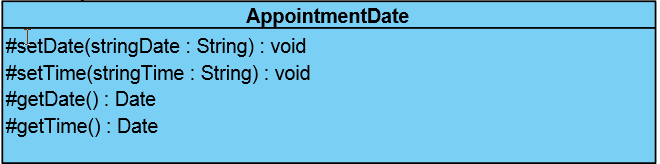
\includegraphics[scale = .5]{res/umlClasses/AppointmentDate.png}
	\centering
\end{figure}
AppointmentDate legt fest wie Datum und Uhrzeit formatiert werden.
\begin{enumerate}
	\item protected setDate(stringDate: String)\\
		Ein Datum festlegen.
	\item protected setTime(stringTime: String)\\
		Eine Uhrzeit festlegen.
	\item protected getDate():Date \\
		Das Datum zurückgeben.
	\item protected getTime():Date \\
		Die Uhrzeit zurückgeben.
\end{enumerate}

\textbf{AppointmentDestination}
\begin{figure}[H]
	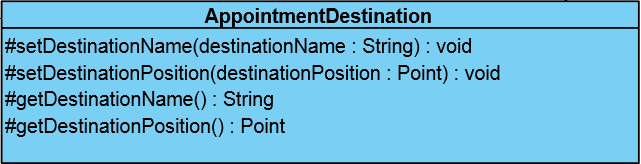
\includegraphics[scale = .5]{res/umlClasses/AppointmentDestination.png}
	\centering
\end{figure}
AppointmentDestination legt fest wie Name und Position des Zielortes definiert sind.
\begin{enumerate}
	\item protected setDestinationName(destinationName:String)\\
		Den Zielort über den Namen/ die Adresse bestimmen.
	\item protected setDestinationPosition(destinationPosition:Point)\\
		Den Zielort über eine Position auf der Karte bestimmen.
	\item protected getDestinationName():String \\
		Den Zielortnamen zurückgeben.
	\item protected getDestinationPosition():Point \\
		Die Zielortposition zurückgeben.
\end{enumerate}


\subsubsection{ClientController}

\textbf{NetworkIntentService}

\paragraph{Database}

\textbf{Services}
Die folgenden Service Klassen stellen die grundlegenden Funktionen zur Verfügung, mit welchen auf die Daten der in den Innenklassen von FeedReaderContract definierten Tabellen der Datenbank zugegriffen werden kann. Dabei können Daten hinzugefügt (insert), gelesen (read), gelöscht (delete) und verändert (update) werden.
Weitere Details dazu, wie die jeweilige Datenbanken aufgebaut sind, finden sie in FeedEntryGroup, FeedEntryUser, FeedEntryAppointment, FeedEntryAllocation.

\begin{figure}[H]
	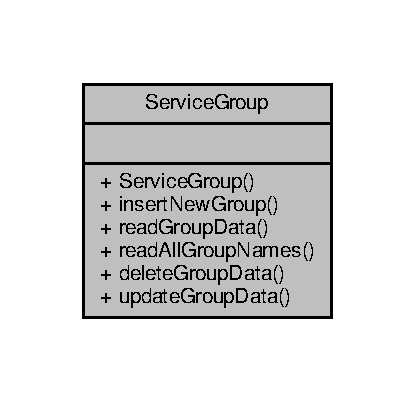
\includegraphics[scale = 1]{res/umlClasses/service_group__coll__graph.pdf}
	\centering
\end{figure}
In der Datenbank auf die ServiceGroup zugreift, werden die Gruppen gespeichert und ob der aktuelle Nutzer der Go-App für diese spezielle Gruppe seinen Go-Button aktiviert hat oder nicht. 
\begin{enumerate}
	\item public ServiceGroup(context: Context)\\
		Konstruktor, dem den Kontext der Applikation mitgegeben wird.
	\item public insertNewGroup(groupClient: GroupClient):boolean\\
		Eine neue Gruppe wird der Datenbank hinzugefügt und der GoStatus des Erstellers auf false gesetzt.
	\item public readGroupData(groupID: int):GroupClient \\
		Informationen über Gruppenname und GoStatus lesen. 
	\item public readAllGroupNames():List<String>\\
		Alle Gruppen in denen der aktuelle Benutzer Mitglied ist werden zurückgegeben.
	\item public deleteGroupData(groupID: int):boolean\\
		Eine Gruppe wird aus der Datenbank gelöscht.
	\item public updateGroupData(groupClient: GroupClient ):boolean\\
		Gruppendaten werden aktualisiert, wenn sich der Gruppenname oder der GoStatus ändert.
\end{enumerate}

\begin{figure}[H]
	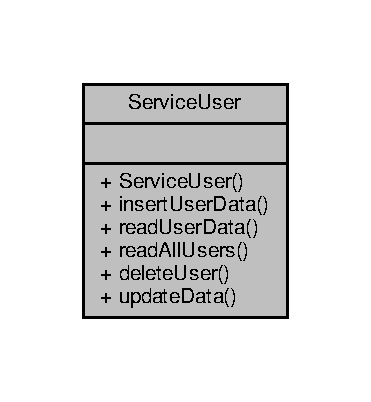
\includegraphics[scale = 1]{res/umlClasses/service_user__coll__graph.pdf}
	\centering
\end{figure}
In der Datenbank auf die ServiceUser zugreift ist der Name und die zuletzt bekannte Position des Benutzers gespeichert, welche bei neuen Informationen angepasst werden. 
\begin{enumerate}
	\item public ServiceUser(context: Context)\\
		Konstruktor, dem den Kontext der Applikation mitgegeben wird.
	\item public insertUserData(UserDecorator user):boolean\\
		Ein neuer Benutzer wird der Datenbank hinzugefügt, sobald dieser mit dem aktuellen Benutzer in einer Gruppe ist.
	\item public readUserData(userID: int):UserDecorator\\
		Inforamtionen über Benutzername und Position eines Benutzers können gelesen werden.
	\item public readAllUsers():List<UserDecorator> \\
		Alle Benutzernamen mit denen der aktuelle Benutzer in einer Gruppe ist lesen.
	\item public deleteUser(userID: int):boolean\\
		Einen Benutzer von der Datenbank entfernen.
	\item public updateData(userID: int):boolean\\
		Benutzerdaten anpassen, wenn sich Name oder Position geändert haben.
\end{enumerate}

\begin{figure}[H]
	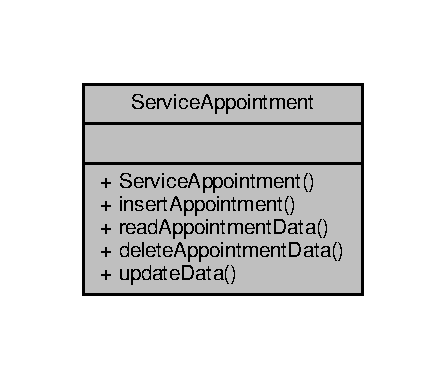
\includegraphics[scale = 1]{res/umlClasses/service_appointment__coll__graph.pdf}
	\centering
\end{figure}
In der Datenbank auf die ServiceAppointment zugreift, wird zu jeder Gruppe das aktuelle Treffen gespeichert und verändert, sobald ein neues existiert.
\begin{enumerate}
	\item public ServiceAppointment(context: Context)\\
		Konstruktor, dem den Kontext der Applikation mitgegeben wird.
	\item public insertAppointment(groupID: int, appointment: Appointment):boolean\\
		Wird aufgerufen wenn eine neue Gruppe erstellt wird. Dabei wird ein default Appointment initialisiert.
	\item public readAppointmentData(groupID: int):Appointment \\
		Informationen über Datum, Uhrzeit, Zielortname und Zielortposition können abgerufen werden.
	\item public deleteAppointmentData(groupID: int):boolean \\
		Wenn eine Gruppe gelöscht wird, wir auch das dazugehörige Appointment gelöscht.
	\item public updateData(groupID: int, appointment: Appointment):boolean \\
		Das Appointment wird angepasst, sobald es geändert wird.
\end{enumerate}

\begin{figure}[H]
	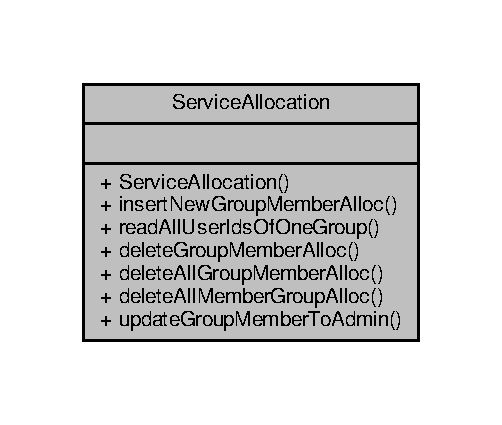
\includegraphics[scale = 1]{res/umlClasses/service_allocation__coll__graph.pdf} 
	\centering
\end{figure}
In der Datenbank auf die ServiceAllocation zugreift, wird die Verbindung zwischen Gruppen und Gruppenmitgliedern bzw. Administratoren gespeichert. 
\begin{enumerate}
	\item public (context: Context):ServiceAllocation\\
		Konstruktor, dem den Kontext der Applikation mitgegeben wird.
	\item public insertNewGroupMemberAlloc(groupID: int , userID: int):boolean\\
		Wenn ein neues Mitglied einer Gruppe hinzugefügt wird, dann wird diese Verbindung hier eingetragen.
	\item public readAllUserIdsOfOneGroup(groupID: int ):List<Integer> \\
		Um alle Mitglieder einer Gruppe zu bekommen, müssen dafür alle Benutzer Id's mit derselben Gruppen Id zurückgegeben werden.
	\item public deleteGroupMemberAlloc(groupid: int, userId: int):boolean \\
		Wird ein Gruppenmitglied aus einer Gruppe entfernt, so wird auch die Verbindung von diesem zur Gruppe gelöscht.
	\item public deleteAllGroupMemberAlloc(groupId: int):boolean \\
		Wird eine Gruppe gelöscht, so werden alle Verbindungen zu Benutzern dieser Gruppe gelöscht.
	\item public updateGroupMemberToAdmin(groupId: int , userID: int):boolean \\
		Wird ein Gruppenmitglied zum Administrator gemacht, dann wird dies in der Datenbank angepasst.
\end{enumerate}
	

\paragraph{ObjectStructure}

In Account- und GroupHandler werden allgemeine Funktionen definiert, die nicht selbst vom GroupClient oder von Unterklassen von UserComponent ausgeführt werden können, sondern eine übergeordnete Position benötigen.

\textbf{AccountHandler}
\begin{figure}[H]
	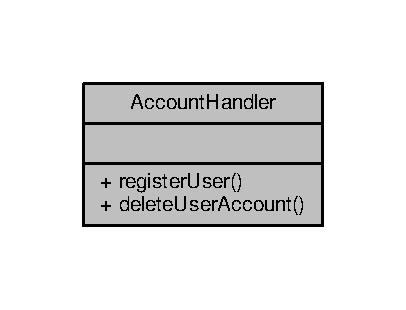
\includegraphics[scale = 1]{res/umlClasses/account_handler__coll__graph.pdf}
	\centering
\end{figure}
Die AccountHandler Klasse handelt das Registrieren und löschen vom aktuellen Benutzer ab.
\begin{enumerate}
	\item public registerUser(userName: String, deviceID: String)\\
		Ein neuer Benutzer registriert sich mit einem Namen und seiner Gerätenummer. Dieser wird zunächst als SimpleUser Objekt angelegt und mit der Gerätenummer auf dem Server gespeichert, um Missbrauch zu verhindern.
	\item public deleteUserAccount(user: UserDecorator)\\
		Löscht ein Benutzer seinen Account, wird er von der Datenbank gelöscht.
\end{enumerate}

\textbf{GroupHandler}
\begin{figure}[H]
	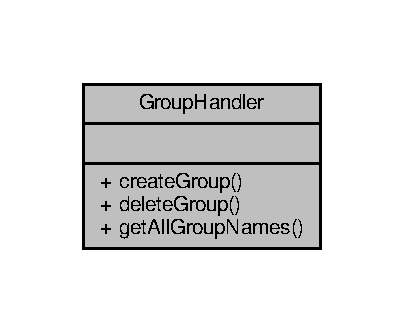
\includegraphics[scale = 1]{res/umlClasses/group_handler__coll__graph.pdf}
	\centering
\end{figure}
Die GroupHandler Klasse handelt das Erstellen und Löschen von Gruppen ab.
\begin{enumerate}
	\item public createGroup(groupName: String, user: UserDecorator)\\
		Eine neue Gruppe wird erstellt, mit einem eindeutigen Gruppennamen und mit dem Ersteller als Administrator.
	\item public deleteGroup(GroupClient groupClient)\\
		Eine Gruppe wird gelöscht und alle ihre Mitglieder entfernt.
\end{enumerate}



\subsection{Serverseitig}



\newpage
\section{Sequenzdiagramme}
Beschreibung von charakteristischen Abläufen anhand von Sequenzdiagrammen. Beispielsweise bieten sich Testszenarien aus dem Pflichtenheft hier an. Wir empfehlen Sequenzdiagramme möglichst früh zu erstellen, dann dabei werden die Schnittstellen zwischen Packages und Klassen klar.
\subsection{Client-Server-Kommunikation}
\subsection{Weiteres Sequendiagramm}
hier würde sich vielleicht noch Gruppe erstellen anbieten, da zum einen eine Gruppe erstellt wird und zum anderen gleichzeitig ein Mitglied als Admin hinzugefügt wird
\newpage
\section{Änderungen zum Pflichtenheft}

Änderungen zum Pflichtenheft, bspw. gekürzte Wunschkriterien.

-Benutzer und Gruppen nach Inaktivität löschen
-Benachrichtigung bei Gruppenaktivität
-



%Erfahrungsgemäßer Umfang:
%100 Seiten, primär Klassenbeschreibungen
%40–80 Klassen ohne Interfaces
%Möglicherweise weitere UML-Diagrammarten?
%Formale Spezifikation von Kernkomponenten?

%Auch nicht zu vergessen sind Dinge die nicht im UML auftauchen. Bilder, SQL-Schema, JSONSchema,
%Tools wie ein Leveleditor, etc.

\end{document}